         \chapter{Rational numbers}
    \setcounter{figure}{1}
    \setcounter{subfigure}{1}
    \label{m38348}
    \section{ Introduction}
            \nopagebreak
            \label{m38348*cid2} $ \hspace{-5pt}\begin{array}{cccccccccccc}   
\includegraphics[width=0.75cm]{col11306.imgs/summary_video.png} &   \end{array} $ \hspace{2 pt}\raisebox{-5 pt}{} {(section shortcode: MG10033 )} \par 
      \label{m38348*id62184}As described in  Review of past work (Section~), a number is a way of representing quantity. The numbers that will be used in high school are all real numbers, but there are many different ways of writing any single real number.\par 
      \label{m38348*id62191}This chapter describes \textsl{rational numbers}.\par \label{m38348*eip-195}
    \setcounter{subfigure}{0}
	\begin{figure}[H] % horizontal\label{m38348*circuits-1}
    \textnormal{Khan Academy video on Integers and Rational Numbers}\vspace{.1in} \nopagebreak
  \label{m38348*yt-media1}\label{m38348*yt-video1}
            \raisebox{-5 pt}{ 
\includegraphics[width=0.5cm]{col11306.imgs/summary_www.png}} { (Video:  MG10034 )}
      \vspace{2pt}
    \vspace{.1in}
 \end{figure}       \par 
    \section{ The Big Picture of Numbers}
            \nopagebreak
            \label{m38348*cid3} $ \hspace{-5pt}\begin{array}{cccccccccccc}   \end{array} $ \hspace{2 pt}\raisebox{-5 pt}{
\includegraphics[width=0.5cm]{col11306.imgs/summary_www.png}} {(section shortcode: MG10035 )} \par 
      \label{m38348*id62547}
    \setcounter{subfigure}{0}
	\begin{figure}[H] % horizontal\label{m38348*id62548}
    \begin{center}
    \label{m38348*id62548!!!underscore!!!media}\label{m38348*id62548!!!underscore!!!printimage}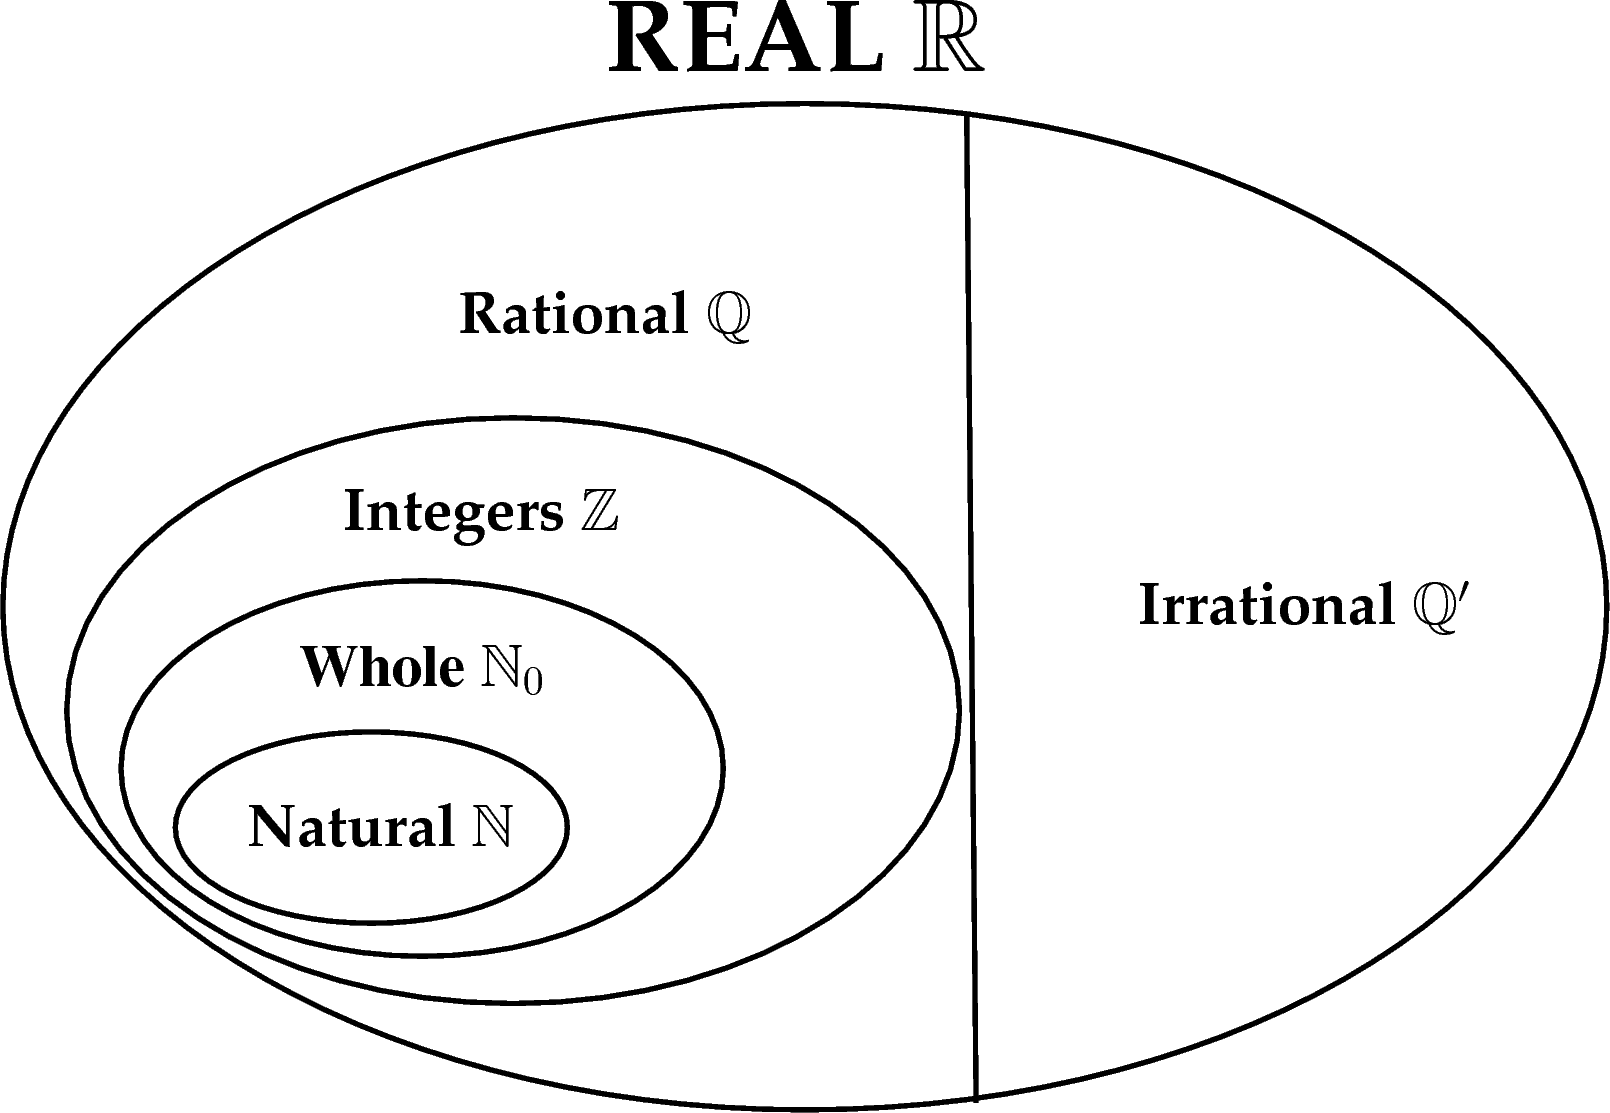
\includegraphics{col11306.imgs/m38348_MG10C3_001.png} % m38348;MG10C3\_001.png;;;6.0;8.5;
      \vspace{2pt}
    \vspace{.1in}
    \end{center}
 \end{figure}       
      \par 
      \label{m38348*id62554}The term whole number does not have a consistent definition. Various authors use
it in many different ways. We use the following definitions:\par 
      \label{m38348*id62559}\begin{itemize}[noitemsep]
            \label{m38348*uid1}\item natural numbers are (1, 2, 3, ...)
\label{m38348*uid2}\item whole numbers are (0, 1, 2, 3, ...)
\label{m38348*uid3}\item integers are (... -3, -2, -1, 0, 1, 2, 3, ....)
\end{itemize}
    \section{ Definition}
            \nopagebreak
            \label{m38348*cid4} $ \hspace{-5pt}\begin{array}{cccccccccccc}   \end{array} $ \hspace{2 pt}\raisebox{-5 pt}{
\includegraphics[width=0.5cm]{col11306.imgs/summary_www.png}} {(section shortcode: MG10036 )} \par 
      \label{m38348*id62607}The following numbers are all rational numbers.\par 
      \label{m38348*uid4}\nopagebreak\noindent{}
        \settowidth{\mymathboxwidth}{\begin{equation}
    \frac{10}{1},\frac{21}{7},\frac{-1}{-3},\frac{10}{20},\frac{-3}{6}\tag{4.1}
      \end{equation}
    }
    \typeout{Columnwidth = \the\columnwidth}\typeout{math as usual width = \the\mymathboxwidth}
    \ifthenelse{\lengthtest{\mymathboxwidth < \columnwidth}}{% if the math fits, do it again, for real
    \begin{equation}
    \frac{10}{1},\frac{21}{7},\frac{-1}{-3},\frac{10}{20},\frac{-3}{6}\tag{4.1}
      \end{equation}
    }{% else, if it doesn't fit
    \setlength{\mymathboxwidth}{\columnwidth}
      \addtolength{\mymathboxwidth}{-48pt}
    \par\vspace{12pt}\noindent\begin{minipage}{\columnwidth}
    \parbox[t]{\mymathboxwidth}{\large$
    \frac{10}{1},\frac{21}{7},\frac{-1}{-3},\frac{10}{20},\frac{-3}{6}$}\hfill
    \parbox[t]{48pt}{\raggedleft 
    (4.1)}
    \end{minipage}\vspace{12pt}\par
    }% end of conditional for this bit of math
    \typeout{math as usual width = \the\mymathboxwidth}
      \label{m38348*id62687}You can see that all denominators and all numerators are integers.\par 
\label{m38348*fhsst!!!underscore!!!id138}\begin{definition}
	  \begin{tabular*}{15 cm}{m{15 mm}m{}}
	\hspace*{-50pt}  
\includegraphics[width=0.5in]{col11306.imgs/psflag2.png}   & \Definition{   \label{id2489628}\textbf{ Rational Number }} { \label{m38348*meaningfhsst!!!underscore!!!id138}
      \label{m38348*id62709}A rational number is any number which can be written as:\par 
      \label{m38348*uid6}\nopagebreak\noindent{}
        \settowidth{\mymathboxwidth}{\begin{equation}
    \frac{a}{b}\tag{4.2}
      \end{equation}
    }
    \typeout{Columnwidth = \the\columnwidth}\typeout{math as usual width = \the\mymathboxwidth}
    \ifthenelse{\lengthtest{\mymathboxwidth < \columnwidth}}{% if the math fits, do it again, for real
    \begin{equation}
    \frac{a}{b}\tag{4.2}
      \end{equation}
    }{% else, if it doesn't fit
    \setlength{\mymathboxwidth}{\columnwidth}
      \addtolength{\mymathboxwidth}{-48pt}
    \par\vspace{12pt}\noindent\begin{minipage}{\columnwidth}
    \parbox[t]{\mymathboxwidth}{\large$
    \frac{a}{b}$}\hfill
    \parbox[t]{48pt}{\raggedleft 
    (4.2)}
    \end{minipage}\vspace{12pt}\par
    }% end of conditional for this bit of math
    \typeout{math as usual width = \the\mymathboxwidth}
      \label{m38348*id62732}where $a$ and $b$ are integers and $b\ne 0$. \par 
       } 
      \end{tabular*}
      \end{definition}
\label{m38348*eip-761}Note that because we can write $\frac{a}{-b}$
as $\frac{-a}{b}$
(in other words, one can always find an equivalent rational expression where $b\greatthan{}0$) mathematicians typically define rational numbers not as both $a$ and $b$ being integers, but rather that $a$ is an integer and $b$ is a natural number. This avoids having to worry about zero in the denominator. \par \label{m38348*notfhsst!!!underscore!!!id150}
\begin{tabular}{cc}
	   \hspace*{-50pt}\raisebox{-8 mm}{ 
\includegraphics[width=0.5in]{col11306.imgs/pstip2.png}  }& 
	\begin{minipage}{0.85\textwidth}
	\begin{note}
      {tip: }Only fractions which have a numerator and a denominator (that is not 0) that are integers
are rational numbers.
	\end{note}
	\end{minipage}
	\end{tabular}
	\par
      \label{m38348*id62778}This means that all integers are rational numbers, because they can be written with a denominator of 1.\par 
      \label{m38348*id62782}Therefore\par 
      \label{m38348*uid7}\nopagebreak\noindent{}
        \settowidth{\mymathboxwidth}{\begin{equation}
    \frac{\sqrt{2}}{7},\frac{\pi }{20}\tag{4.3}
      \end{equation}
    }
    \typeout{Columnwidth = \the\columnwidth}\typeout{math as usual width = \the\mymathboxwidth}
    \ifthenelse{\lengthtest{\mymathboxwidth < \columnwidth}}{% if the math fits, do it again, for real
    \begin{equation}
    \frac{\sqrt{2}}{7},\frac{\pi }{20}\tag{4.3}
      \end{equation}
    }{% else, if it doesn't fit
    \setlength{\mymathboxwidth}{\columnwidth}
      \addtolength{\mymathboxwidth}{-48pt}
    \par\vspace{12pt}\noindent\begin{minipage}{\columnwidth}
    \parbox[t]{\mymathboxwidth}{\large$
    \frac{\sqrt{2}}{7},\frac{\pi }{20}$}\hfill
    \parbox[t]{48pt}{\raggedleft 
    (4.3)}
    \end{minipage}\vspace{12pt}\par
    }% end of conditional for this bit of math
    \typeout{math as usual width = \the\mymathboxwidth}
      \label{m38348*id62817}are \textbf{not examples} of rational numbers, because in each case, either the numerator or the denominator is not an integer.\par 
      \label{m38348*id62829}A number may not be written as an integer divided by another integer, but may still
be a rational number. This is because the results may be expressed
as an integer divided by an integer. The rule is, if a number can be written
as a fraction of integers, it is rational even if it can also be written in another
way as well. Here are two examples that might not look like rational numbers
at first glance but are because there are equivalent forms that are expressed as an
integer divided by another integer:\par 
      \label{m38348*uid8}\nopagebreak\noindent{}\settowidth{\mymathboxwidth}{\begin{equation}
    \frac{-1,33}{-3}=\frac{133}{300},\frac{-3}{6,39}=\frac{-300}{639}=\frac{-100}{213}\tag{4.4}
      \end{equation}
    }
    \typeout{Columnwidth = \the\columnwidth}\typeout{math as usual width = \the\mymathboxwidth}
    \ifthenelse{\lengthtest{\mymathboxwidth < \columnwidth}}{% if the math fits, do it again, for real
    \begin{equation}
    \frac{-1,33}{-3}=\frac{133}{300},\frac{-3}{6,39}=\frac{-300}{639}=\frac{-100}{213}\tag{4.4}
      \end{equation}
    }{% else, if it doesn't fit
    \setlength{\mymathboxwidth}{\columnwidth}
      \addtolength{\mymathboxwidth}{-48pt}
    \par\vspace{12pt}\noindent\begin{minipage}{\columnwidth}
    \parbox[t]{\mymathboxwidth}{\large$
    \frac{-1,33}{-3}=\frac{133}{300},\frac{-3}{6,39}=\frac{-300}{639}=\frac{-100}{213}$}\hfill
    \parbox[t]{48pt}{\raggedleft 
    (4.4)}
    \end{minipage}\vspace{12pt}\par
    }% end of conditional for this bit of math
    \typeout{math as usual width = \the\mymathboxwidth}
\label{m38348*secfhsst!!!underscore!!!id232}
            \subsection{ Rational Numbers }
            \nopagebreak
            \label{m38348*id63121}\begin{enumerate}[noitemsep, label=\textbf{\arabic*}. ] 
            \label{m38348*uid9}\item If $a$ is an integer, $b$ is an integer and $c$ is irrational, which of the following are rational numbers? 
\label{m38348*id734}\begin{enumerate}[noitemsep, label=\textbf{\alph*}. ] 
            \item $\frac{5}{6}$\newline
    \item $\frac{a}{3}$\newline
    \item $\frac{b}{2}$\newline
    \item $\frac{1}{c}$\end{enumerate}
        \label{m38348*uid10}\item If $\frac{a}{1}$ is a rational number, which of the following are valid values for $a$?\label{m38348*id7432}\begin{enumerate}[noitemsep, label=\textbf{\alph*}. ] 
            \item 1\item $-10$\item $\sqrt{2}$\item $2,1$\end{enumerate}
        \end{enumerate}
\par \raisebox{-5 pt}{
\includegraphics[width=0.5cm]{col11306.imgs/summary_www.png}} Find the answers with the shortcodes:
 \par \begin{tabular}[h]{cccccc}
 (1.) l35  &  (2.) l3N  & \end{tabular}
    \section{ Forms of Rational Numbers}
            \nopagebreak
            \label{m38348*cid5} $ \hspace{-5pt}\begin{array}{cccccccccccc}   \end{array} $ \hspace{2 pt}\raisebox{-5 pt}{
\includegraphics[width=0.5cm]{col11306.imgs/summary_www.png}} {(section shortcode: MG10037 )} \par 
      \label{m38348*id63345}All integers and fractions with integer numerators and denominators are rational numbers. There are two more forms of rational numbers.\par 
\label{m38348*secfhsst!!!underscore!!!id245}
            \subsection{  Investigation : Decimal Numbers }
            \nopagebreak
      \label{m38348*id63357}You can write the rational number
$\frac{1}{2}$ as the decimal number 0,5. Write the following numbers as
decimals:\par 
      \label{m38348*id63375}\begin{enumerate}[noitemsep, label=\textbf{\arabic*}. ] 
            \label{m38348*uid11}\item 
          $\frac{1}{4}$
        \label{m38348*uid12}\item 
          $\frac{1}{10}$
        \label{m38348*uid13}\item 
          $\frac{2}{5}$
        \label{m38348*uid14}\item 
          $\frac{1}{100}$
        \label{m38348*uid15}\item 
          $\frac{2}{3}$
        \end{enumerate}
      \label{m38348*id63486}Do the numbers after the decimal comma end or do they continue? If they continue, is there a repeating pattern to the numbers? \par 
      \label{m38348*id63495}You can write a rational number as a decimal number. Two types of decimal numbers can be written as rational numbers:\par 
      \label{m38348*id63500}\begin{enumerate}[noitemsep, label=\textbf{\arabic*}. ] 
            \label{m38348*uid16}\item decimal numbers that end or \textsl{terminate}, for example the fraction $\frac{4}{10}$ can be written as 0,4.
\label{m38348*uid17}\item decimal numbers that have a repeating pattern of numbers, for example the fraction $\frac{1}{3}$ can be written as 
$0,\dot{3}$. 
The dot represents recurring $3$'s i.e.,
$0,333...=0,\dot{3}$.
\end{enumerate}
      \label{m38348*id63576}For example, the rational number $\frac{5}{6}$ can be written in decimal notation as $0,8\dot{3}$ and similarly, the decimal number 0,25 can be written as a rational number as $\frac{1}{4}$.\par 
\label{m38348*notfhsst!!!underscore!!!id301}
\begin{tabular}{cc}
	   \hspace*{-50pt}\raisebox{-8 mm}{ 
\includegraphics[width=0.5in]{col11306.imgs/pstip2.png}  }& 
	\begin{minipage}{0.85\textwidth}
	\begin{note}
      {tip: }You can use a bar over the repeated numbers to indicate that the decimal is a repeating decimal.
	\end{note}
	\end{minipage}
	\end{tabular}
	\par
    \section{ Converting Terminating Decimals into Rational Numbers}
            \nopagebreak
            \label{m38348*cid6} $ \hspace{-5pt}\begin{array}{cccccccccccc}   \end{array} $ \hspace{2 pt}\raisebox{-5 pt}{
\includegraphics[width=0.5cm]{col11306.imgs/summary_www.png}} {(section shortcode: MG10038 )} \par 
      \label{m38348*id63646}A decimal number has an integer part and a fractional part. For example $10,589$ has an integer part of 10 and a fractional part of $0,589$ because $10+0,589=10,589$. The fractional part can be written as a rational number, i.e. with a numerator and a denominator that are integers.\par 
      \label{m38348*id63704}Each digit after the decimal point is a fraction with a denominator in increasing powers of ten. For example:\par 
      \label{m38348*id63708}\begin{itemize}[noitemsep]
            \label{m38348*uid18}\item $\frac{1}{10}$ is $0,1$\label{m38348*uid19}\item $\frac{1}{100}$ is $0,01$\end{itemize}
      \label{m38348*id63781}This means that:\par 
      \label{m38348*id63784}\nopagebreak\noindent{}\settowidth{\mymathboxwidth}{\begin{equation}
    \begin{array}{ccc}\hfill 10,589& =& 10+\frac{5}{10}+\frac{8}{100}+\frac{9}{1000}\hfill \\ & =& 10\frac{589}{1000}\hfill \\ & =& \frac{10589}{1000}\hfill \end{array}\tag{4.5}
      \end{equation}
    }
    \typeout{Columnwidth = \the\columnwidth}\typeout{math as usual width = \the\mymathboxwidth}
    \ifthenelse{\lengthtest{\mymathboxwidth < \columnwidth}}{% if the math fits, do it again, for real
    \begin{equation}
    \begin{array}{ccc}\hfill 10,589& =& 10+\frac{5}{10}+\frac{8}{100}+\frac{9}{1000}\hfill \\ & =& 10\frac{589}{1000}\hfill \\ & =& \frac{10589}{1000}\hfill \end{array}\tag{4.5}
      \end{equation}
    }{% else, if it doesn't fit
    \setlength{\mymathboxwidth}{\columnwidth}
      \addtolength{\mymathboxwidth}{-48pt}
    \par\vspace{12pt}\noindent\begin{minipage}{\columnwidth}
    \parbox[t]{\mymathboxwidth}{\large$
    10,589=10+\frac{5}{10}+\frac{8}{100}+\frac{9}{1000}=10\frac{589}{1000}=\frac{10589}{1000}$}\hfill
    \parbox[t]{48pt}{\raggedleft 
    (4.5)}
    \end{minipage}\vspace{12pt}\par
    }% end of conditional for this bit of math
    \typeout{math as usual width = \the\mymathboxwidth}
\label{m38348*secfhsst!!!underscore!!!id378}
            \subsection{  Fractions }
            \nopagebreak
      \label{m38348*id63882}\begin{enumerate}[noitemsep, label=\textbf{\arabic*}. ] 
            \label{m38348*uid20}\item Write the following as fractions:\label{m38348*id7322}\begin{enumerate}[noitemsep, label=\textbf{\alph*}. ] 
            \item $0,1$\item $0,12$\item $0,58$\item $0,2589$\end{enumerate}
        \end{enumerate}
\par \raisebox{-5 pt}{
\includegraphics[width=0.5cm]{col11306.imgs/summary_www.png}} Find the answers with the shortcodes:
 \par \begin{tabular}[h]{cccccc}
 (1.) l3R  & \end{tabular}
    \section{ Converting Repeating Decimals into Rational Numbers}
            \nopagebreak
            \label{m38348*cid7} $ \hspace{-5pt}\begin{array}{cccccccccccc}   \end{array} $ \hspace{2 pt}\raisebox{-5 pt}{
\includegraphics[width=0.5cm]{col11306.imgs/summary_www.png}} {(section shortcode: MG10039 )} \par 
      \label{m38348*id63993}When the decimal is a repeating decimal, a bit more work is needed to write the fractional part of the decimal number as a fraction. We will explain by means of an example.\par 
      \label{m38348*id63998}If we wish to write $0,\dot{3}$ in the form $\frac{a}{b}$ (where $a$ and $b$ are integers) then we would proceed as follows
\par 
      \label{m38348*uid21}\nopagebreak\noindent{}\settowidth{\mymathboxwidth}{\begin{equation}
    \begin{array}{cccc}\hfill x& =& 0,33333...\hfill & \\ \hfill 10x& =& 3,33333...\hfill & \text{multiply}\phantom{\rule{4.pt}{0ex}}\text{by}\phantom{\rule{4.pt}{0ex}}\text{10}\phantom{\rule{4.pt}{0ex}}\text{on}\phantom{\rule{4.pt}{0ex}}\text{both}\phantom{\rule{4.pt}{0ex}}\text{sides}\hfill \\ \hfill 9x& =& 3\hfill & \text{(}\text{subtracting}\phantom{\rule{4.pt}{0ex}}\text{the}\phantom{\rule{4.pt}{0ex}}\text{second}\phantom{\rule{4.pt}{0ex}}\text{equation}\phantom{\rule{4.pt}{0ex}}\text{from}\phantom{\rule{4.pt}{0ex}}\text{the}\phantom{\rule{4.pt}{0ex}}\text{first}\phantom{\rule{4.pt}{0ex}}\text{equation}\text{)}\hfill \\ \hfill x& =& \frac{3}{9}=\frac{1}{3}\hfill & \end{array}\tag{4.6}
      \end{equation}
    }
    \typeout{Columnwidth = \the\columnwidth}\typeout{math as usual width = \the\mymathboxwidth}
    \ifthenelse{\lengthtest{\mymathboxwidth < \columnwidth}}{% if the math fits, do it again, for real
    \begin{equation}
    \begin{array}{cccc}\hfill x& =& 0,33333...\hfill & \\ \hfill 10x& =& 3,33333...\hfill & \text{multiply}\phantom{\rule{4.pt}{0ex}}\text{by}\phantom{\rule{4.pt}{0ex}}\text{10}\phantom{\rule{4.pt}{0ex}}\text{on}\phantom{\rule{4.pt}{0ex}}\text{both}\phantom{\rule{4.pt}{0ex}}\text{sides}\hfill \\ \hfill 9x& =& 3\hfill & \text{(}\text{subtracting}\phantom{\rule{4.pt}{0ex}}\text{the}\phantom{\rule{4.pt}{0ex}}\text{second}\phantom{\rule{4.pt}{0ex}}\text{equation}\phantom{\rule{4.pt}{0ex}}\text{from}\phantom{\rule{4.pt}{0ex}}\text{the}\phantom{\rule{4.pt}{0ex}}\text{first}\phantom{\rule{4.pt}{0ex}}\text{equation}\text{)}\hfill \\ \hfill x& =& \frac{3}{9}=\frac{1}{3}\hfill & \end{array}\tag{4.6}
      \end{equation}
    }{% else, if it doesn't fit
    \setlength{\mymathboxwidth}{\columnwidth}
      \addtolength{\mymathboxwidth}{-48pt}
    \par\vspace{12pt}\noindent\begin{minipage}{\columnwidth}
    \parbox[t]{\mymathboxwidth}{\large$
    x=0,33333...10x=3,33333...\text{multiply}\phantom{\rule{4.pt}{0ex}}\text{by}\phantom{\rule{4.pt}{0ex}}\text{10}\phantom{\rule{4.pt}{0ex}}\text{on}\phantom{\rule{4.pt}{0ex}}\text{both}\phantom{\rule{4.pt}{0ex}}\text{sides}9x=3\text{(}\text{subtracting}\phantom{\rule{4.pt}{0ex}}\text{the}\phantom{\rule{4.pt}{0ex}}\text{second}\phantom{\rule{4.pt}{0ex}}\text{equation}\phantom{\rule{4.pt}{0ex}}\text{from}\phantom{\rule{4.pt}{0ex}}\text{the}\phantom{\rule{4.pt}{0ex}}\text{first}\phantom{\rule{4.pt}{0ex}}\text{equation}\text{)}x=\frac{3}{9}=\frac{1}{3}$}\hfill
    \parbox[t]{48pt}{\raggedleft 
    (4.6)}
    \end{minipage}\vspace{12pt}\par
    }% end of conditional for this bit of math
    \typeout{math as usual width = \the\mymathboxwidth}
      \label{m38348*id64237}And another example would be to write 
$5,\dot{4}\dot{3}\dot{2}$ 
as a rational fraction.
\par 
      \label{m38348*uid22}\nopagebreak\noindent{}\settowidth{\mymathboxwidth}{\begin{equation}
    \begin{array}{cccc}\hfill x& =& 5,432432432...\hfill & \\ \hfill 1000x& =& 5432,432432432...\hfill & \text{multiply by\hspace{0.17em}}\phantom{\rule{4.pt}{0ex}}\text{1000}\phantom{\rule{4.pt}{0ex}}\text{on both sides}\\ \hfill \\ \hfill 999x& =& 5427\hfill & \text{(}\text{subtracting the second equation from the first equation}\text{)}\\ \hfill x& =& \frac{5427}{999}=\frac{201}{37}\hfill & \end{array}\tag{4.7}
      \end{equation}
    }
    \typeout{Columnwidth = \the\columnwidth}\typeout{math as usual width = \the\mymathboxwidth}
    \ifthenelse{\lengthtest{\mymathboxwidth < \columnwidth}}{% if the math fits, do it again, for real
    \begin{equation}
    \begin{array}{cccc}\hfill x& =& 5,432432432...\hfill & \\ \hfill 1000x& =& 5432,432432432...\hfill & \text{multiply by\hspace{0.17em}}\phantom{\rule{4.pt}{0ex}}\text{1000}\phantom{\rule{4.pt}{0ex}}\text{on both sides}\\ \hfill \\ \hfill 999x& =& 5427\hfill & \text{(}\text{subtracting the second equation from the first equation}\text{)}\\ \hfill x& =& \frac{5427}{999}=\frac{201}{37}\hfill & \end{array}\tag{4.7}
      \end{equation}
    }{% else, if it doesn't fit
    \setlength{\mymathboxwidth}{\columnwidth}
      \addtolength{\mymathboxwidth}{-48pt}
    \par\vspace{12pt}\noindent\begin{minipage}{\columnwidth}
    \parbox[t]{\mymathboxwidth}{\large$
    x=5,432432432...1000x=5432,432432432...\text{multiply by\hspace{0.17em}}\phantom{\rule{4.pt}{0ex}}\text{1000}\phantom{\rule{4.pt}{0ex}}\text{on both sides}999x=5427\text{(}\text{subtracting the second equation from the first equation}\text{)}x=\frac{5427}{999}=\frac{201}{37}$}\hfill
    \parbox[t]{48pt}{\raggedleft 
    (4.7)}
    \end{minipage}\vspace{12pt}\par
    }% end of conditional for this bit of math
    \typeout{math as usual width = \the\mymathboxwidth}
      \label{m38348*id64459}For the first example, the decimal was multiplied by 10 and for the second example, the decimal was multiplied by 1000. This is because for the first example there was only one digit (i.e. 3) recurring, while for the second example there were three digits (i.e. 432) recurring.\par 
      \label{m38348*id64465}In general, if you have one digit recurring, then multiply by 10. If you have two digits recurring, then multiply by 100. If you have three digits recurring, then multiply by 1000. Can you spot the pattern yet?\par 
      \label{m38348*id64470}The number of zeros is the same as the number of recurring digits.\par 
      \label{m38348*id64474}Not all decimal numbers can be written as rational numbers. Why? Irrational decimal numbers like 
$\sqrt{2}=1,4142135...$
cannot be written with an integer numerator and denominator, because they do not have a pattern of recurring digits. However, when possible, you should try to use rational numbers or fractions instead of decimals.\par 
\label{m38348*secfhsst!!!underscore!!!id606}
            \subsection{  Repeated Decimal Notation }
            \nopagebreak
      \label{m38348*id64513}\begin{enumerate}[noitemsep, label=\textbf{\arabic*}. ] 
            \label{m38348*uid23}\item Write the following using the repeated decimal notation:
\label{m38348*id64529}\begin{enumerate}[noitemsep, label=\textbf{\alph*}. ] 
            \label{m38348*uid24}\item $0,11111111...$\label{m38348*uid25}\item $0,1212121212...$\label{m38348*uid26}\item $0,123123123123...$\label{m38348*uid27}\item $0,11414541454145...$\end{enumerate}
        \label{m38348*uid28}\item Write the following in decimal form, using the repeated decimal notation:
\label{m38348*id64650}\begin{enumerate}[noitemsep, label=\textbf{\alph*}. ] 
            \label{m38348*uid29}\item $\frac{2}{3}$\label{m38348*uid30}\item $1\frac{3}{11}$\label{m38348*uid31}\item $4\frac{5}{6}$\label{m38348*uid32}\item $2\frac{1}{9}$\end{enumerate}
        \label{m38348*uid33}\item Write the following decimals in fractional form:
\label{m38348*id64767}\begin{enumerate}[noitemsep, label=\textbf{\alph*}. ] 
            \label{m38348*uid34}\item $0,633\dot{3}$\label{m38348*uid35}\item $5,3131\overline{31}$\label{m38348*uid36}\item $0,99999\dot{9}$\end{enumerate}
        \end{enumerate}
\par \raisebox{-5 pt}{
\includegraphics[width=0.5cm]{col11306.imgs/summary_www.png}} Find the answers with the shortcodes:
 \par \begin{tabular}[h]{cccccc}
 (1.) l3U  &  (2.) l3n  &  (3.) l3Q  & \end{tabular}
    \section{ Summary}
            \nopagebreak
            \label{m38348*cid8} $ \hspace{-5pt}\begin{array}{cccccccccccc}   \end{array} $ \hspace{2 pt}\raisebox{-5 pt}{
\includegraphics[width=0.5cm]{col11306.imgs/summary_www.png}} {(section shortcode: MG10040 )} \par \label{m38348*eip-280}\begin{itemize}[noitemsep, label=\textbullet{}]
            \item Real numbers can be either rational or irrational.\item  A rational number is any number which can be written as 
$\frac{a}{b}$
where $a$ and $b$ are integers and $b\ne 0$\item The following are rational numbers:
      \label{m38348*id64890}\begin{enumerate}[noitemsep, label=\textbf{\alph*}. ] 
            \label{m38348*uid37}\item Fractions with both denominator and numerator as integers.
\label{m38348*uid38}\item Integers.
\label{m38348*uid39}\item Decimal numbers that end.
\label{m38348*uid40}\item Decimal numbers that repeat.
\end{enumerate}
        \end{itemize}
    \section{ End of Chapter Exercises}
            \nopagebreak
            \label{m38348*cid9} $ \hspace{-5pt}\begin{array}{cccccccccccc}   \end{array} $ \hspace{2 pt}\raisebox{-5 pt}{
\includegraphics[width=0.5cm]{col11306.imgs/summary_www.png}} {(section shortcode: MG10041 )} \par \label{m38348*id64954}\begin{enumerate}[noitemsep, label=\textbf{\arabic*}. ] 
            \label{m38348*uid41}\item If $a$ is an integer, $b$ is an integer and $c$ is irrational, which of the following are rational numbers?
\label{m38348*id64997}\begin{enumerate}[noitemsep, label=\textbf{\alph*}. ] 
            \label{m38348*uid42}\item $\frac{5}{6}$\label{m38348*uid43}\item $\frac{a}{3}$\label{m38348*uid44}\item $\frac{b}{2}$\label{m38348*uid45}\item $\frac{1}{c}$
\end{enumerate}
\label{m38348*uid46}\item Write each decimal as a simple fraction:
\label{m38348*id65104}\begin{enumerate}[noitemsep, label=\textbf{\alph*}. ] 
            \label{m38348*uid47}\item $0,5$\label{m38348*uid48}\item $0,12$\label{m38348*uid49}\item $0,6$\label{m38348*uid50}\item $1,59$\label{m38348*uid51}\item $12,27\dot{7}$
\end{enumerate}
\label{m38348*uid52}\item Show that the decimal $3,21\dot{1}\dot{8}$ is a rational number.
\newline
\label{m38348*uid53}\item Express $0,7\dot{8}$ as a fraction $\frac{a}{b}$ where $a,b\in \mathbb{Z}$ (show all working).
\newline
\end{enumerate}
  \label{m38348**end}
\par \raisebox{-5 pt}{
\includegraphics[width=0.5cm]{col11306.imgs/summary_www.png}} Find the answers with the shortcodes:
 \par \begin{tabular}[h]{cccccc}
 (1.) l3v  &  (2.) l3f  &  (3.) l3G  &  (4.) lOf  & \end{tabular}
